%% ============================================================================
%% Artigo P2 PDI -- template da disciplina (template_pdi_com_tabelas_segmentacao.tex)
%% Elsevier - Results in Engineering, classe elsarticle, duas colunas (5p)
%% Tabelas em tables/ geradas por scripts/08_artigo_pdi.py; figuras em figures/.
%% Compilacao: latexmk -pdf main.tex
%% ============================================================================
\documentclass[final,5p,times,twocolumn]{elsarticle}

%% --- Pacotes essenciais (template) ---
\usepackage[utf8]{inputenc}
\usepackage[T1]{fontenc}
\usepackage{amsmath,amssymb,amsfonts}
\usepackage{graphicx}
\usepackage{booktabs}
\usepackage{tabularx}
\usepackage{multirow}
\usepackage{array}
\usepackage{microtype}
\usepackage{lineno}
\usepackage[colorlinks=true,linkcolor=blue,citecolor=blue,urlcolor=blue]{hyperref}
%% --- Acrescimos deste artigo ---
\usepackage{tikz}
\usetikzlibrary{positioning,arrows.meta,calc}

\biboptions{sort&compress}
\journal{Results in Engineering}
\modulolinenumbers[5]

\newcolumntype{L}[1]{>{\raggedright\arraybackslash}p{#1}}
\newcolumntype{Y}{>{\raggedright\arraybackslash}X}

\graphicspath{{figures/}}
%% Posicionamento de floats: permite mais tabelas/figuras por pagina em duas colunas
\renewcommand{\topfraction}{0.9}
\renewcommand{\dbltopfraction}{0.9}
\renewcommand{\bottomfraction}{0.8}
\renewcommand{\textfraction}{0.07}
\renewcommand{\floatpagefraction}{0.75}
\renewcommand{\dblfloatpagefraction}{0.75}
\setcounter{topnumber}{4}
\setcounter{dbltopnumber}{4}
\setcounter{totalnumber}{6}
\newcommand{\ind}{\mathbf{1}}

\begin{document}

%% ============================================================================
%% CABECALHO (FRONTMATTER)
%% ============================================================================
\begin{frontmatter}

\title{Temporal segmentation of active-reaction regions in the Gray-Scott system of The Well: pre-processing, architectures and post-processing}

\author[a]{Andre Luis Aguiar do Nascimento}
\ead{andre.aguiar@discente.ufma.br}

\author[a]{Joao Guilherme Miranda Lago}
\ead{jglago10@gmail.com}

\author[a]{Wesley dos Santos Gatinho}
\ead{wesley.gatinho@discente.ufma.br}

\affiliation[a]{%
    organization={Universidade Federal do Maranh\~ao (UFMA)},
    city={S\~ao Lu\'is},
    postcode={65080-805},
    country={Brazil}
}

\begin{abstract}
Reaction-diffusion systems describe chemical reactors, the spreading of reacting substances and biological pattern formation, and quantifying where their structures are and how they evolve requires segmenting the concentration fields over time. This study evaluates how pre-processing, segmentation architecture and post-processing affect the segmentation of the active-reaction regions of the two-dimensional Gray-Scott system of The Well, under a protocol shared by a class of Digital Image Processing. The ground truth thresholds the autocatalytic species $B$ with Otsu's method at a mid-simulation snapshot, and the networks recover it from the substrate $A$ at the native $128\times128$ resolution. Ten pre-processing methods, three architectures (U-Net, SegFormer and Mask2Former, 20 training epochs each) and five post-processing methods were applied to all 1,200 trajectories, giving 150 combinations of the protocol matrix plus 48 baseline rows. On 120 test trajectories, U-Net reached a Dice of 0.953 without pre- or post-processing, against 0.892 for SegFormer, 0.768 for Mask2Former and 0.888 for Otsu thresholding of $A$. Pre-processing changed Dice by at most 1.37 percentage points, and temporal filtering lowered it by 8.6 to 11.3 points. The largest gains came from the random initial snapshot: once that snapshot was excluded, threshold optimization lowered the Dice of U-Net and SegFormer. In this dataset, the output resolution of the architecture weighed more than the techniques applied around it, and selecting configurations by mean Dice was sensitive to a single frame without physical information.
\end{abstract}

\begin{keyword}
Gray-Scott model \sep
reaction-diffusion \sep
semantic segmentation \sep
U-Net \sep
SegFormer \sep
Mask2Former \sep
The Well
\end{keyword}

\end{frontmatter}

%% ============================================================================
%% SUMARIO (CONTENTS)
%% ============================================================================
\setcounter{tocdepth}{2}
\tableofcontents
\vspace{1em}

%% ============================================================================
\section{Introduction}\label{sec:intro}

Reaction-diffusion systems describe substances that spread in space while they react with each other. When the species diffuse at different rates, diffusion, which alone smooths any perturbation, can destabilize a homogeneous medium and give rise to spots, labyrinths and waves that emerge without external control. Turing~\cite{turing1952} proposed this mechanism to explain morphogenesis; the same framework has been used to describe biological patterns~\cite{kondo2010,murray2003} and was observed experimentally in chemical reactors~\cite{lee1993}. The Gray-Scott model is the minimal form of this phenomenon: two species, one cubic autocatalytic reaction and two control parameters are enough to generate qualitatively distinct stationary and dynamic patterns~\cite{gray1983,pearson1993}. Analyzing such a pattern requires more than observing the concentration field. It requires answering where the structures of interest are and how they evolve over time, which means turning the continuous field into regions, that is, segmenting it.

The Well collection provides simulations of the Gray-Scott system, among other physical systems, for the development of machine-learning methods~\cite{ohana2024well}. In that collection, the reference models are neural surrogates, such as the Fourier Neural Operator, that predict the next states of the field~\cite{li2021fno,brunton2020}. Prediction, however, neither locates the structures nor measures their formation, migration or extinction. Semantic segmentation by deep networks, established in natural and medical images~\cite{long2015fcn,ronneberger2015unet,xie2021segformer,cheng2022mask2former}, provides that representation, but its behavior on simulated fields, without texture, on a periodic domain and with structures that appear and vanish, is less documented. In addition, classical steps that precede the network, such as normalizations and filters, or follow it, such as thresholding and morphology, are often applied without measuring whether and why they change the segmentation.

In this context, this study evaluates the effect of pre-processing, segmentation architecture and post-processing on the temporal segmentation of the active-reaction regions of the Gray-Scott system of The Well. The study follows a protocol shared by a Digital Image Processing class, in which each participant applies the same experiment to a different two-dimensional dataset: ten pre-processing methods, three architectures and five post-processing methods, an input of at most 128 pixels along the largest axis without upscaling, a subset of at most 25~GB per dataset and 20 training epochs. The experiment is organized in four conditions: the architecture alone, pre-processing followed by the architecture, the architecture followed by post-processing, and the combination of the three stages. Four research questions guide the study: (RQ1) how U-Net, SegFormer and Mask2Former compare with each other and with a learning-free reference; (RQ2) to what extent pre-processing changes the segmentation of each architecture; (RQ3) to what extent post-processing changes it; and (RQ4) whether the masks follow the temporal evolution of the structures, including their formation and extinction.

The contribution is empirical and descriptive: a physically defined ground truth, the evaluation of the 150 combinations of the protocol and of their baseline rows with class-wise, temporal and cost metrics, paired analyses that isolate the effect of each technique, and a sensitivity analysis to the initial snapshot. No new architecture is proposed. The scope of the results is limited by one random seed per training, by a ground truth obtained by thresholding rather than by expert annotation, and by the adaptation of the Mask2Former training to the available budget (Section~\ref{subsec:architectures}).

The paper is organized as follows. Section~\ref{sec:sec2} presents the Gray-Scott system, its applications and the dataset. Section~\ref{sec:sec3} reviews the segmentation architectures, and Section~\ref{sec:sec4} the pre- and post-processing techniques. The evaluation metrics are defined in Section~\ref{sec:sec5}. Section~\ref{sec:experimental} describes the experimental protocol and reports the comparative results, which are discussed in Section~\ref{sec:sec6}. Finally, concluding remarks are provided in Section~\ref{sec:conclusions}.

%% ============================================================================
\section{The Gray-Scott reaction-diffusion system}\label{sec:sec2}

\subsection{Reaction-diffusion and the Turing mechanism}\label{subsec:turing}

A reaction-diffusion system with two species of concentrations $u(\mathbf{x},t)$ and $v(\mathbf{x},t)$ reads
\begin{equation}\label{eq:rd}
\frac{\partial u}{\partial t} = D_u \nabla^2 u + f(u,v), \qquad
\frac{\partial v}{\partial t} = D_v \nabla^2 v + g(u,v),
\end{equation}
where $\nabla^2$ is the Laplacian, responsible for spatial spreading according to Fick's law, and $f$ and $g$ represent the local kinetics. Let $(u^*,v^*)$ be a homogeneous steady state and $\mathbf{J}$ the Jacobian of the kinetics at that state. A perturbation proportional to $e^{\lambda t+i\mathbf{q}\cdot\mathbf{x}}$ grows at the rate given by the eigenvalues of $\mathbf{J}-q^2\mathbf{D}$, with $\mathbf{D}=\mathrm{diag}(D_u,D_v)$. Turing~\cite{turing1952} showed that a state that is stable without diffusion ($\operatorname{tr}\mathbf{J}<0$ and $\det\mathbf{J}>0$) can be destabilized by it if
\begin{equation}\label{eq:turing}
h(q^2)=D_uD_v q^4-(D_u J_{22} + D_v J_{11})\,q^2+\det\mathbf{J} < 0
\end{equation}
for some $q$, which only happens when the species diffuse at sufficiently different rates. The band of unstable wavenumbers sets the characteristic length of the pattern, independently of the size of the domain~\cite{murray2003}.

\subsection{The Gray-Scott model}\label{subsec:gsmodel}

The Gray-Scott model describes a continuously fed isothermal reactor in which a substrate $A$ is converted by the autocatalytic step $A+2B\rightarrow 3B$ and the autocatalyst decays as $B\rightarrow P$, $P$ being an inert product~\cite{gray1983,gray1984}. In dimensionless, spatially extended form,
\begin{subequations}\label{eq:gs}
\begin{align}
\frac{\partial A}{\partial t} &= \delta_A\nabla^2 A - A B^2 + F\,(1-A), \label{eq:gsA}\\
\frac{\partial B}{\partial t} &= \delta_B\nabla^2 B + A B^2 - (F+k)\,B, \label{eq:gsB}
\end{align}
\end{subequations}
where $AB^2$ is the reaction rate, which consumes $A$ and produces $B$, $F$ is the feed rate of $A$, and $k$ is the kill rate of $B$. The trivial state $(A,B)=(1,0)$ always exists and is linearly stable, with eigenvalues $-F$ and $-(F+k)$; it represents a reactor in which the autocatalyst has disappeared. The non-trivial states satisfy $AB=F+k$ and $F(1-A)=(F+k)B$, so that
\begin{equation}\label{eq:gsfixed}
B_\pm=\frac{F\pm\sqrt{F^2-4F(F+k)^2}}{2(F+k)},\qquad A_\pm=\frac{F+k}{B_\pm},
\end{equation}
which exist only below the saddle-node curve $k=\tfrac12\sqrt{F}-F$ of the $(F,k)$ plane, with Jacobian
\begin{equation}\label{eq:gsjac}
\mathbf{J}=\begin{pmatrix} -B^{*2}-F & -2(F+k)\\ B^{*2} & F+k\end{pmatrix}.
\end{equation}
Pearson~\cite{pearson1993} showed that, near these boundaries, localized perturbations of the trivial state evolve into self-replicating spots, traveling pulses and labyrinths, depending on the region of the $(F,k)$ plane. Two consequences matter for segmentation: small changes of $(F,k)$ change the pattern qualitatively, and for some parameters the pattern collapses to the trivial state, so that all structures disappear.

Eqs.~\eqref{eq:gsA} and~\eqref{eq:gsB} also explain the relation between the two fields used in this study. Where the reaction is active, $B$ is high, and $A$ is consumed, which makes the fields anti-correlated. Because $A$ diffuses twice as fast as $B$ in the simulations used, the depletion region of $A$ around a structure is wider and smoother than the structure itself. The boundary $\{B=\tau\}$ therefore does not coincide with an iso-line of $A$, and recovering it from $A$ is a non-linear, non-local inverse problem.

\subsection{Where the Gray-Scott system applies}\label{subsec:applications}

In chemical reaction engineering, the model was formulated to explain multistability, ignition, extinction and oscillations in continuous reactors with cubic autocatalysis~\cite{gray1983,gray1984}, and its spatial form describes gel reactors, in which the predicted self-replicating spots were observed~\cite{lee1993}; the region $\{B>\tau\}$ is then the region where the reaction is ignited, and its area over time, including its collapse, relates to reactor yield. In industrial safety, an accidentally released gas spreads by diffusion while it reacts with air, and emergency planning simulates such scenarios, for example, an ammonia leak, to delimit at each instant the region where the concentration exceeds a threshold, which is the operation studied here. In biology, Turing-type models explain pigmentation patterns and the spacing of follicles~\cite{kondo2010,murray2003}, and segmentation converts the pattern into the number, size and spacing of its structures. In scientific machine learning, The Well uses this system to benchmark neural surrogates~\cite{ohana2024well}, and segmentation provides a structure-level diagnostic of whether patterns are preserved in long rollouts.

\subsection{The \texttt{gray\_scott\_reaction\_diffusion} dataset}\label{subsec:dataset}

The dataset has 1,200 trajectories: six parameter sets, which correspond to pattern regimes, each with 200 random initial conditions, split by trajectory into 160, 20 and 20 for training, validation and test~\cite{ohana2024well}. The regimes are \textit{gliders} ($F=0.014$, $k=0.054$), \textit{bubbles} ($0.098$, $0.057$), \textit{maze} ($0.029$, $0.057$), \textit{worms} ($0.058$, $0.065$), \textit{spirals} ($0.018$, $0.051$) and \textit{spots} ($0.030$, $0.062$). All simulations use $\delta_A=2\times10^{-5}$ and $\delta_B=10^{-5}$ on the periodic square $[-1,1]^2$ with $128\times128$ points, a Fourier pseudo-spectral discretization, and fourth-order exponential time differencing (ETDRK4)~\cite{cox2002,kassam2005}. Snapshots are stored every 10 time units up to $t=10{,}000$, giving 1,001 snapshots per trajectory and 154~GB; time is indexed here by the snapshot number $n\in\{0,\dots,1000\}$. Several \textit{glider} trajectories reach a homogeneous steady state, a fact handled in the construction of the ground truth.

%% ============================================================================
\section{Segmentation architectures}\label{sec:sec3}

Given a field $X\in\mathbb{R}^{H\times W\times C}$, semantic segmentation assigns a label to each pixel; in this study, background or structure. Fully convolutional networks made this task an end-to-end learning problem~\cite{long2015fcn}, and the three architectures evaluated represent distinct design families.

\subsection{U-Net}\label{subsec:unet}

U-Net is a symmetric encoder-decoder~\cite{ronneberger2015unet}. The encoder progressively reduces the resolution and increases the number of channels, and the decoder recovers the original resolution. At each scale, a skip connection concatenates the decoder map with the encoder map of the same resolution, re-injecting spatial detail lost in the reduction. Here the encoder is a ResNet-34 pre-trained on ImageNet~\cite{he2016resnet,deng2009imagenet}, whose residual blocks compute $\mathbf{y}=\mathcal{F}(\mathbf{x})+\mathbf{x}$, for a total of 24.4 million parameters. The output is a logit map $z$ at the input resolution, and the structure probability is $p=\sigma(z)$.

\subsection{SegFormer}\label{subsec:segformer}

Transformers replace convolution with self-attention, $\mathrm{Attn}(Q,K,V)=\mathrm{softmax}(QK^\top/\sqrt{d})\,V$, in which each token interacts with all others~\cite{vaswani2017}; the Vision Transformer applies this operation to image patches~\cite{dosovitskiy2021vit}. SegFormer adapts the idea to dense prediction with a hierarchical encoder, the Mix Transformer, inspired by PVT~\cite{wang2021pvt,xie2021segformer}, which produces maps at $1/4$, $1/8$, $1/16$ and $1/32$ of the input resolution. Its components are overlapping patch merging by strided convolutions; efficient self-attention, in which keys and values are spatially reduced by a ratio $R$, lowering the cost from $O(N^2)$ to $O(N^2/R)$; the Mix-FFN, $\mathbf{x}_{out}=\mathrm{MLP}(\mathrm{GELU}(\mathrm{Conv}_{3\times3}(\mathrm{MLP}(\mathbf{x}_{in}))))+\mathbf{x}_{in}$, whose convolution provides positional information without explicit positional encoding; and an all-MLP decoder that projects the four scales, upsamples them to $1/4$ of the resolution and fuses them. The MiT-B2 variant pre-trained on ImageNet-1k was used, with 27.3 million parameters.

\subsection{Mask2Former}\label{subsec:mask2former}

MaskFormer reformulated segmentation as mask classification: instead of classifying each pixel, the model predicts a set of $N$ pairs $\{(p_i,m_i)\}_{i=1}^N$, each formed by a distribution $p_i$ over $K$ classes plus a ``no object'' class and by a binary mask $m_i$~\cite{cheng2021maskformer}, in the line of DETR~\cite{carion2020detr}. Mask2Former combines a backbone, here Swin-T with shifted-window attention~\cite{liu2021swin}, a pixel decoder with multi-scale deformable attention~\cite{zhu2021deformable} and a Transformer decoder whose $N$ learnable queries use masked attention~\cite{cheng2022mask2former},
\begin{equation}\label{eq:maskedattn}
\mathbf{X}_l=\mathrm{softmax}(\mathcal{M}_{l-1}+\mathbf{Q}_l\mathbf{K}_l^\top)\mathbf{V}_l+\mathbf{X}_{l-1},
\end{equation}
with $\mathcal{M}_{l-1}(x,y)=0$ where $m_{l-1}(x,y)\geq 0.5$ and $-\infty$ otherwise, so that each query attends only to the region of its current mask. In training, predictions are matched one-to-one to ground-truth segments by the Hungarian algorithm~\cite{kuhn1955}, and the loss is $\mathcal{L}=\lambda_{ce}\mathcal{L}_{ce}+\lambda_{bce}\mathcal{L}_{bce}+\lambda_{dice}\mathcal{L}_{dice}$ with $\lambda=(2,5,5)$; in the original recipe, this loss is also applied to the output of every intermediate decoder layer, which is called deep supervision. In semantic inference, the score of class $c$ at each pixel is $\sum_i p_i(c)\,m_i(x,y)$. The Swin-T model trained on ADE20K~\cite{zhou2017ade} was used, with 47.4 million parameters and $N=100$ queries; its classifier was replaced by a two-class one.

\subsection{Output resolution}\label{subsec:outres}

U-Net predicts at the input resolution, whereas SegFormer and Mask2Former predict at $1/4$ of it. For a $128\times128$ input, the output of these two architectures has $32\times32$ cells and is bilinearly interpolated to $128\times128$. This difference is a property of the architectures and is revisited in Section~\ref{sec:sec6}.

%% ============================================================================
\section{Pre-processing and post-processing}\label{sec:sec4}

\subsection{Pre-processing}\label{subsec:pretheory}

Pre-processing modifies the field before the network. Normalizations change the values using training statistics: the z-score computes $x'=(x-\mu)/\sigma$; RMS normalization divides by the root mean square, $x'=x/\sqrt{\overline{x^2}}$, preserving zero and the shape of the distribution; robust scaling computes $x'=(x-\mathrm{med})/\mathrm{IQR}$, which is little affected by extreme values; min-max normalization computes $x'=(x-x_{\min})/(x_{\max}-x_{\min})$; and percentile clipping saturates the values outside $[p_1,p_{99}]$. Spatial filters change the structure of the field~\cite{gonzalez2018}. Gaussian smoothing, $x'=G_\sigma * x$, multiplies the spectrum by $e^{-\sigma^2q^2/2}$; the median filter replaces each pixel by the median of its neighborhood; the bilateral filter weights neighbors by spatial distance and intensity difference, smoothing homogeneous regions while preserving edges~\cite{tomasi1998}; Perona-Malik anisotropic diffusion solves
\begin{equation}\label{eq:pm}
\partial_\tau I=\nabla\cdot\big(c(|\nabla I|)\nabla I\big),\qquad c(s)=e^{-(s/\kappa)^2},
\end{equation}
which inhibits diffusion across strong gradients~\cite{perona1990}; and wavelet denoising soft-thresholds the detail coefficients, $\eta_\lambda(w)=\mathrm{sign}(w)\max(|w|-\lambda,0)$, with the adaptive BayesShrink threshold $\lambda=\hat\sigma_n^2/\hat\sigma_x$~\cite{donoho1994,chang2000,daubechies1992}.

\subsection{Post-processing}\label{subsec:posttheory}

Post-processing turns the probability map $P(x,y)\in[0,1]$ into the final mask. Threshold optimization chooses $\tau$ in $\ind[P>\tau]$ to correct the calibration bias of the network. Morphological opening, $\gamma_B(X)=(X\ominus B)\oplus B$, removes objects smaller than the structuring element $B$, and closing, $\varphi_B(X)=(X\oplus B)\ominus B$, fills narrow gaps and reconnects nearby parts~\cite{serra1982,soille2003}. Connected-component filtering removes regions whose area is below a minimum, under the hypothesis that very small components are noise. Temporal consistency filtering takes the median of the probabilities of $w$ consecutive snapshots of the same trajectory before thresholding, reducing oscillations between frames.

%% ============================================================================
\section{Evaluation metrics}\label{sec:sec5}

\subsection{Overlap and class-wise metrics}\label{subsec:overlap}

Let $TP$, $FP$, $FN$ and $TN$ be the numbers of true-positive, false-positive, false-negative and true-negative pixels of a frame. Following recommendations for the validation of segmentations~\cite{taha2015,maierhein2024}, the main metrics for the structure class are
\begin{equation}\label{eq:iou}
\mathrm{IoU}=\frac{TP}{TP+FP+FN}, \qquad \mathrm{Dice}=\frac{2TP}{2TP+FP+FN},
\end{equation}
where the Jaccard index (IoU) and the Dice coefficient derive from measures of association between sets~\cite{jaccard1912,dice1945}. Precision, $TP/(TP+FP)$, and recall, $TP/(TP+FN)$, are also reported, together with the background-class metrics $\mathrm{IoU}_{bg}=TN/(TN+FP+FN)$ and $\mathrm{Dice}_{bg}=2TN/(2TN+FP+FN)$ and the mIoU, the mean IoU of the two classes. Frames in which prediction and ground truth are both empty, as after the extinction of a pattern, receive IoU and Dice equal to 1. The metrics are computed per frame, averaged per trajectory and then across trajectories. Since IoU and Dice are related by $\mathrm{Dice}=2\,\mathrm{IoU}/(1+\mathrm{IoU})$ only frame by frame, their means over frames can rank two configurations differently when the per-frame scores are very unequal.

\subsection{Temporal metrics}\label{subsec:temporal}

Three metrics compare the dynamics of the predicted masks with those of the ground truth along each trajectory sampled at $t_0<\dots<t_T$. The area-variation error is $\mathrm{AVE}=\frac{1}{T}\sum_j|\Delta a_{pred}(t_j)-\Delta a_{gt}(t_j)|$, where $a(t)$ is the segmented fraction of the domain, in percent, and $\Delta a(t_j)=a(t_j)-a(t_{j-1})$. The centroid displacement error (CDE) operates per structure, since the global centroid of a pattern that fills the periodic domain is ill-defined: connected components that touch across opposite borders are merged, the centroid of each structure is a circular mean, $\bar y=\frac{H}{2\pi}\operatorname{atan2}(\sum\sin\theta_y,\sum\cos\theta_y)$ with $\theta_y=2\pi y/H$, and each ground-truth centroid is paired with the nearest predicted centroid, and vice versa, using the periodic distance $d_{per}$:
\begin{equation}\label{eq:cde}
\mathrm{CDE}(t)=\frac12\Big[\frac{1}{|\mathcal{G}|}\sum_{g\in\mathcal{G}}\min_{p\in\mathcal{P}}d_{per}(g,p)+\frac{1}{|\mathcal{P}|}\sum_{p\in\mathcal{P}}\min_{g\in\mathcal{G}}d_{per}(g,p)\Big].
\end{equation}
The temporal consistency $\mathrm{TC}=\frac{1}{T}\sum_j\mathrm{IoU}(\hat M(t_j),\hat M(t_{j-1}))$ measures the overlap between consecutive masks, and the error $\mathrm{TCE}=|\mathrm{TC}_{pred}-\mathrm{TC}_{gt}|$ compares it with that of the ground truth, since a moving pattern has low consistency without this being an error.

\subsection{Cost and uncertainty}\label{subsec:cost}

Latency is the mean time to segment one $128\times128$ frame with batch 1, after 30 warm-up passes and over 200 passes, measured after all training runs with a dedicated GPU; memory is the peak GPU memory allocated. Because frames of a trajectory are correlated, the resampling unit is the trajectory: 95\% confidence intervals were obtained by a non-parametric bootstrap~\cite{efron1993} with 2,000 resamples of the test trajectories, stratified by regime. The effect of each technique was estimated by the paired difference $\Delta_i=\mathrm{Dice}_i(\text{technique})-\mathrm{Dice}_i(\text{architecture alone})$ on each trajectory $i$, whose mean received the same procedure; an effect is called distinguishable from zero when its interval excludes zero.

%% ============================================================================
%% SECAO EXPERIMENTAL (template da disciplina)
%% ============================================================================
\section{Experimental protocol and comparative results}\label{sec:experimental}

\subsection{Datasets and physical segmentation targets}\label{subsec:datasets}

Table~\ref{tab:datasets} states the physical target and the ground-truth rule of this dataset, fixed before training. The structures of interest are the regions where the autocatalytic reaction is active, that is, where the concentration of $B$ is high. For each trajectory $i$, the snapshot $n_{ref}=500$, at which the patterns of the regimes are developed, was taken, and the Otsu threshold of $B_i(\cdot,n_{ref})$, which maximizes the between-class variance~\cite{otsu1979,sezgin2004}, was computed:
\begin{equation}\label{eq:otsu}
\tau_i=\arg\max_{\tau}\;\omega_0(\tau)\,\omega_1(\tau)\,[\mu_0(\tau)-\mu_1(\tau)]^2 .
\end{equation}
The ground truth of every snapshot is $M_i(x,y,n)=\ind[B_i(x,y,n)>\tau_i]$. The fixed threshold per trajectory anchors the definition of a structure at the characteristic snapshot, so that the masks record how structures emerge from the initial condition, grow, split, migrate or vanish, without the definition adapting to each snapshot.

\begin{table*}[t]
    \centering
    \caption{Dataset of this study and its segmentation target (row of the class table of The Well datasets).}
    \label{tab:datasets}
    \small
    \begin{tabularx}{\textwidth}{L{3.6cm} L{1.65cm} L{2.35cm} Y Y}
        \toprule
        \textbf{Dataset} & \textbf{Grid} & \textbf{Physical system} &
        \textbf{Target} & \textbf{Ground-truth definition / variable} \\
        \midrule
        \texttt{gray\_scott\_reaction\_}\newline\texttt{diffusion} & $128\times128$ & Reaction-diffusion &
        Active-reaction regions (high autocatalyst $B$); network input: substrate $A$ only &
        $M=\ind[B>\tau_i]$, $\tau_i$ = Otsu threshold of $B$ of trajectory $i$ at $n=500$, applied to all snapshots; extinct reference frame ($\max B-\min B\le0.05$): median valid $\tau$ of the regime in training \\
        \bottomrule
    \end{tabularx}
\end{table*}

When the reference snapshot has no contrast, the pattern has collapsed to the trivial state and the Otsu threshold is undefined. This happened in 70 of the 160 training trajectories of \textit{gliders} and 4 of the 160 of \textit{spirals}, plus 12 validation and 9 test trajectories, in agreement with the dataset documentation. For these trajectories, the median valid threshold of the same regime in training was used, so that the masks still delimit the structure while it exists and become empty after the extinction. Table~\ref{tab:regimes} characterizes the regimes.

\begin{table}[t]
    \centering
    \caption{Pattern regimes: mean ground-truth threshold $\bar\tau$, mean structure fraction (fg), trajectories extinct at $n=500$ (all splits), dominant wavelength $\lambda$ of $B$ at $n=500$ and median equivalent diameter $d_{eq}=\sqrt{4a/\pi}$ of the ground-truth structures (training split).}
    \label{tab:regimes}
    \scriptsize
    \setlength{\tabcolsep}{3pt}
    \begin{tabularx}{\columnwidth}{Y c c c c c c c}
        \toprule
        \textbf{Regime} & $F$ & $k$ & $\bar\tau$ & \textbf{fg (\%)} & \textbf{Ext.} & $\lambda$ \textbf{(px)} & $d_{eq}$ \textbf{(px)} \\
        \midrule
        Gliders & 0.014 & 0.054 & 0.110 & 9.2 & 89 & 14.2 & 6.9 \\
        Bubbles & 0.098 & 0.057 & 0.207 & 24.3 & 0 & 14.2 & 5.0 \\
        Maze & 0.029 & 0.057 & 0.163 & 48.0 & 0 & 8.5 & 12.5 \\
        Worms & 0.058 & 0.065 & 0.176 & 23.9 & 0 & 9.8 & 5.4 \\
        Spirals & 0.018 & 0.051 & 0.129 & 31.2 & 6 & 21.3 & 8.8 \\
        Spots & 0.030 & 0.062 & 0.160 & 25.1 & 0 & 8.5 & 5.3 \\
        \bottomrule
    \end{tabularx}
\end{table}

The networks receive only the substrate $A$, never the field $B$ that defines the ground truth; otherwise, the task would reduce to relearning a known threshold. Since the two fields are strongly anti-correlated, a learning-free reference was included: per-frame Otsu thresholding of $A$, $\hat M=\ind[A<\tau_A]$, which shows how much the networks add to that physical relation.

The protocol limits each subset to 25~GB, prioritizing diversity of trajectories and frames. Since the HDF5 files store each field as a contiguous uncompressed array, any frame can be read with an HTTP byte-range request. All 1,200 trajectories of the official split files and 21 snapshots spread over the whole trajectory ($n=0,50,\dots,1000$) were used: 960, 120 and 120 trajectories with 20,160, 2,520 and 2,520 frames, no trajectory shared across splits, in 3.3~GB, with identifiers and dataset revision recorded in a manifest. Using all trajectories keeps the diversity of initial conditions, and the stride of 50 snapshots keeps the training cost comparable to a denser sampling of fewer trajectories. The native grid ($128\times128$, aspect ratio 1:1) is already at the protocol cap, so the field was used without resampling, cropping or padding; at half the resolution, the finest regimes would have about four pixels per period (Table~\ref{tab:regimes}). The protocol's two-resolution pilot does not apply, since a level above 128 pixels would require upscaling.

\subsection{Pre-processing methods}\label{subsec:preprocessing}

Table~\ref{tab:preprocessing} lists the pre-processing methods. The protocol requires a baseline with the chosen standard normalization and no spatial filter. For Gray-Scott, the standard normalization is the model's own non-dimensionalization, in which concentrations are expressed relative to the feed concentration of $A$; the baseline P0 is therefore the dimensionless field without transformation. The filters P6 to P10 were applied to this same input, which separates the effect of normalizations (P1 to P5 against P0) from that of filters (P6 to P10 against P0). Statistics were estimated on the training split only and kept fixed for validation and test. The percentiles of P5 were inspected before use: in training, $p_1=0.252$ and $p_{99}=1.000$, so clipping saturates the low concentrations inside structures and the excess above 1 present only in initial conditions. Filters used periodic padding.

\begin{table*}[t]
    \centering
    \caption{Pre-processing methods and parameters used (statistics from the training split).}
    \label{tab:preprocessing}
    \small
    \begin{tabularx}{\textwidth}{L{0.65cm} L{3.0cm} L{2.35cm} Y Y}
        \toprule
        \textbf{ID} & \textbf{Method} & \textbf{Category} &
        \textbf{Purpose} & \textbf{Parameters used} \\
        \midrule
        P0 & Baseline & Reference input &
        Dimensionless field, no filter & Concentration $A$, native $128\times128$ \\
        P1 & Z-score normalization & Numerical scaling &
        Standardize the input channel & Training mean and standard deviation \\
        P2 & RMS normalization & Numerical scaling &
        Unit RMS, preserving zero & $x/\sqrt{\overline{x^2}}$, training RMS \\
        P3 & Robust normalization & Numerical scaling &
        Reduce sensitivity to extreme values & Training median and interquartile range \\
        P4 & Min-Max normalization & Numerical scaling &
        Map values to $[0,1]$ & Training minimum and maximum \\
        P5 & Percentile clipping & Numerical scaling &
        Limit extreme values & Clip to $[p_1,p_{99}]=[0.252,1.000]$, no rescaling \\
        P6 & Gaussian filter & Spatial filtering &
        Suppress high-frequency variation & $\sigma=1.0$ px, periodic \\
        P7 & Median filter & Spatial filtering &
        Reduce impulsive noise & $3\times3$ window, periodic \\
        P8 & Bilateral filter & Spatial filtering &
        Smooth while retaining edges & $d=5$, $\sigma_{color}=0.1$, $\sigma_{space}=2.0$, periodic \\
        P9 & Anisotropic diffusion & Spatial filtering &
        Smooth while preserving structures & 15 iterations, $\kappa=0.05$, $\gamma=0.2$, exponential conductance \\
        P10 & Wavelet denoising & Multiscale filtering &
        Suppress small wavelet coefficients & Daubechies-4, 3 levels, BayesShrink soft thresholding \\
        \bottomrule
    \end{tabularx}
\end{table*}

\subsection{Segmentation architectures}\label{subsec:architectures}

Table~\ref{tab:architectures} summarizes the three architectures. All started from RGB pre-trained weights, and the first convolution was adapted to the single physical channel by summing its kernels over the color channels, which preserves the response to a gray-level image. Following the protocol, all networks were trained for exactly 20 epochs, one epoch being one pass over the 20,160 training frames with batches of 32 frames (630 iterations), without early stopping; the checkpoint with the best validation Dice, evaluated at the end of each epoch, was kept and its epoch recorded. Optimization used AdamW~\cite{loshchilov2019adamw} with weight decay $10^{-4}$ and learning rates of $3\times10^{-4}$, $2\times10^{-4}$ and $10^{-4}$, one warm-up epoch followed by cosine decay~\cite{loshchilov2017sgdr}, and bfloat16 mixed precision. U-Net and SegFormer minimized binary cross-entropy plus soft Dice~\cite{milletari2016vnet}. Since the Gray-Scott equations are isotropic and the domain is periodic, circular shifts, $90^\circ$ rotations and reflections are exact symmetries of the system and were applied jointly to input and mask as data augmentation.

\begin{table*}[t]
    \centering
    \caption{Deep-learning architectures included in the comparison.}
    \label{tab:architectures}
    \small
    \begin{tabularx}{\textwidth}{L{2.4cm} L{2.55cm} Y Y}
        \toprule
        \textbf{Architecture} & \textbf{Family} & \textbf{Role in the study} &
        \textbf{Implementation details} \\
        \midrule
        U-Net & Convolutional encoder-decoder &
        Convolutional baseline; output at input resolution ($128\times128$) &
        ResNet-34 encoder (ImageNet), 5 stages, skip connections, 1-channel stem, 24.4 M parameters; BCE + soft Dice; lr $3\times10^{-4}$ \\
        \addlinespace
        SegFormer & Hierarchical Transformer &
        Transformer semantic segmentation; output at $1/4$ ($32\times32$) &
        MiT-B2 (ImageNet-1k), all-MLP decoder, 1-channel stem, 27.3 M parameters; BCE + soft Dice; lr $2\times10^{-4}$ \\
        \addlinespace
        Mask2Former & Mask-classification Transformer &
        Mask-based segmentation; output at $1/4$ ($32\times32$) &
        Swin-T backbone (ADE20K), 100 queries, 2 classes, 47.4 M parameters; set loss on the final decoder layer only (no deep supervision); lr $10^{-4}$ \\
        \bottomrule
    \end{tabularx}
\end{table*}

Mask2Former was trained with its set-prediction loss computed only on the final decoder layer, without the deep supervision of the nine intermediate layers; architecture and inference were not changed. The decision was taken after measuring, in the execution environment, 2.67~s per iteration with deep supervision and 0.79~s without it, because the Hungarian matching is solved per sample and per layer on the CPU; with deep supervision, the 11 Mask2Former training runs of 20 epochs would have made the run about three times longer.

\subsection{Post-processing methods}\label{subsec:postprocessing}

Table~\ref{tab:postprocessing} lists the post-processing methods, applied to the stored probability maps without retraining. Their parameters were selected on the validation split by the highest mean Dice and frozen before testing. Morphological operations used periodic padding.

\begin{table*}[t]
    \centering
    \caption{Post-processing methods and parameters (candidate values; the selected value of each configuration is stored with the results).}
    \label{tab:postprocessing}
    \small
    \begin{tabularx}{\textwidth}{L{0.65cm} L{3.0cm} L{2.5cm} Y Y}
        \toprule
        \textbf{ID} & \textbf{Method} & \textbf{Input representation} &
        \textbf{Purpose} & \textbf{Parameters (selected on validation)} \\
        \midrule
        Q0 & Baseline & Probability map &
        Default decision & $\ind[P>0.5]$ \\
        Q1 & Threshold optimization & Probability map &
        Correct calibration bias & $\tau\in\{0.05,\dots,0.95\}$; selected 0.2 for all U-Net and SegFormer inputs \\
        Q2 & Morphological opening & Binary mask &
        Remove small foreground structures & Disk, radius $\in\{1,2\}$ \\
        Q3 & Morphological closing & Binary mask &
        Close small gaps & Disk, radius $\in\{1,2\}$ \\
        Q4 & Connected-component filtering & Component map &
        Remove components below an area & 4-connectivity, $a_{min}\in\{2,4,8,16,32\}$ px; selected 2 to 8 \\
        Q5 & Temporal consistency filtering & Probability sequence &
        Reduce frame-to-frame oscillation & Median over $w\in\{3,5\}$ consecutive sampled snapshots \\
        \bottomrule
    \end{tabularx}
\end{table*}

\subsection{Experimental design and result reporting}\label{subsec:experimental_design}

Fig.~\ref{fig:overview} summarizes the protocol, which is the same for all datasets of the class. For each of the 11 inputs (baseline P0 and P1 to P10) and each of the three architectures, a network was trained, for a total of 33 training runs, and its probabilities on the validation and test splits were stored. The baseline Q0 and the five methods Q1 to Q5 were then applied to the stored probabilities. The result is the $10\times3\times5=150$ combinations of the protocol matrix plus 48 baseline rows without pre- and/or post-processing. Following the class convention, E001 to E150 are P1 to P10 $\times$ architecture $\times$ Q1 to Q5, in the order U-Net, SegFormer and Mask2Former, and E151 to E198 are the baseline rows. For each architecture, the four conditions were selected on the validation split by the highest mean Dice and evaluated once on the test split. Training ran on an NVIDIA RTX A5000 (24~GB) in a container with about seven CPU cores and up to five simultaneous training runs; the full run took about 11.5~h. The code uses PyTorch~\cite{paszke2019pytorch}, Hugging Face Transformers~\cite{wolf2020transformers}, Segmentation Models PyTorch~\cite{iakubovskii2019smp} and scikit-image~\cite{vanderwalt2014skimage}, with seed 42.

\begin{figure*}[t]
\centering
\resizebox{0.86\textwidth}{!}{%
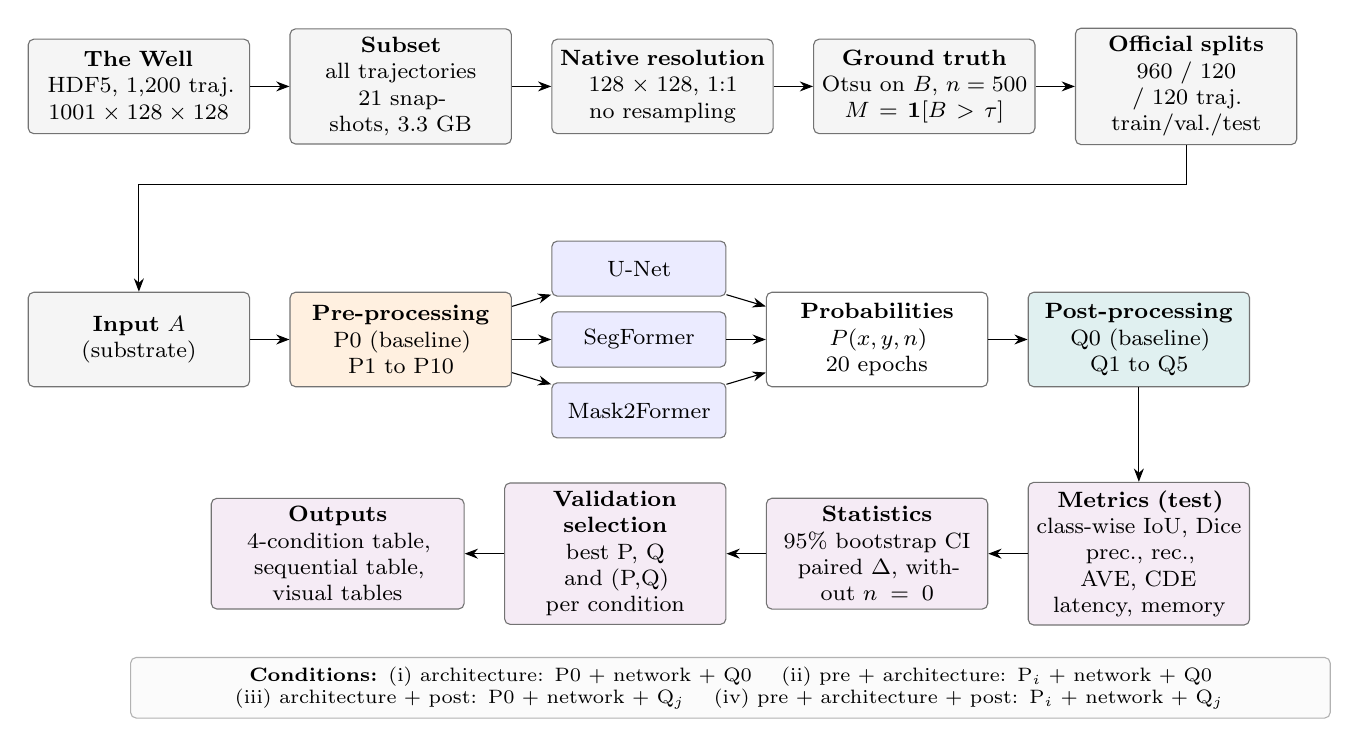
\begin{tikzpicture}[node distance=5mm and 5mm, >=Stealth, font=\footnotesize,
  box/.style={draw=black!55, rounded corners=2pt, align=center, minimum height=12mm, inner sep=3pt, fill=white, text width=26mm},
  data/.style={box, fill=gray!8},
  prep/.style={box, fill=orange!12},
  net/.style={box, fill=blue!8, text width=20mm, minimum height=7mm},
  postp/.style={box, fill=teal!12},
  evalb/.style={box, fill=violet!8}]
\node[data] (well) {\textbf{The Well}\\ HDF5, 1,200 traj.\\ $1001\times128\times128$};
\node[data, right=of well] (sub) {\textbf{Subset}\\ all trajectories\\ 21 snapshots, 3.3 GB};
\node[data, right=of sub] (res) {\textbf{Native resolution}\\ $128\times128$, 1:1\\ no resampling};
\node[data, right=of res] (gt) {\textbf{Ground truth}\\ Otsu on $B$, $n=500$\\ $M=\ind[B>\tau]$};
\node[data, right=of gt] (part) {\textbf{Official splits}\\ 960 / 120 / 120 traj.\\ train/val./test};
\draw[->] (well) -- (sub); \draw[->] (sub) -- (res); \draw[->] (res) -- (gt); \draw[->] (gt) -- (part);
\node[data, below=20mm of well] (inp) {\textbf{Input $A$}\\ (substrate)};
\node[prep, right=of inp] (pre) {\textbf{Pre-processing}\\ P0 (baseline)\\ P1 to P10};
\node[net, right=of pre, yshift=9mm] (u) {U-Net};
\node[net, right=of pre] (s) {SegFormer};
\node[net, right=of pre, yshift=-9mm] (m) {Mask2Former};
\node[box, right=of s] (prob) {\textbf{Probabilities}\\ $P(x,y,n)$\\ 20 epochs};
\node[postp, right=of prob] (posq) {\textbf{Post-processing}\\ Q0 (baseline)\\ Q1 to Q5};
\draw[->] (part.south) |- ++(0,-5mm) -| (inp.north);
\draw[->] (inp) -- (pre); \draw[->] (pre) -- (u); \draw[->] (pre) -- (s); \draw[->] (pre) -- (m);
\draw[->] (u) -- (prob); \draw[->] (s) -- (prob); \draw[->] (m) -- (prob); \draw[->] (prob) -- (posq);
\node[evalb, below=12mm of posq] (met) {\textbf{Metrics (test)}\\ class-wise IoU, Dice\\ prec., rec., AVE, CDE\\ latency, memory};
\node[evalb, left=of met] (est) {\textbf{Statistics}\\ 95\% bootstrap CI\\ paired $\Delta$, without $n=0$};
\node[evalb, left=of est] (sel) {\textbf{Validation selection}\\ best P, Q and (P,Q)\\ per condition};
\node[evalb, left=of sel, text width=30mm] (out) {\textbf{Outputs}\\ 4-condition table,\\ sequential table,\\ visual tables};
\draw[->] (posq) -- (met); \draw[->] (met) -- (est); \draw[->] (est) -- (sel); \draw[->] (sel) -- (out);
\coordinate (mid) at ($(out.south west)!0.5!(met.south east)$);
\node[below=5mm of mid, align=center, font=\scriptsize, draw=black!30, rounded corners=2pt, fill=gray!3, text width=150mm]
  {\textbf{Conditions:} (i) architecture: P0 + network + Q0 \quad (ii) pre + architecture: P$_i$ + network + Q0\\
   (iii) architecture + post: P0 + network + Q$_j$ \quad (iv) pre + architecture + post: P$_i$ + network + Q$_j$};
\end{tikzpicture}}
\caption{Experimental pipeline, common to the datasets of the class: data and ground truth (top), segmentation with 33 trained networks and five post-processing methods applied to the stored probabilities (middle), and evaluation, selection of the four conditions on validation and outputs (bottom).}
\label{fig:overview}
\end{figure*}

Table~\ref{tab:full_results} reports the four conditions of each architecture in the long format of the class, and Table~\ref{tab:architecture_comparison} condenses them. U-Net reached a Dice of 0.953 alone and 0.962 with the selected pair P2+Q1, SegFormer 0.892 alone and at most 0.893 with processing, and Mask2Former 0.768 alone and 0.784 with P5+Q2. The learning-free reference reached 0.888, an interval that overlaps that of SegFormer. Over all snapshots, U-Net therefore exceeds the reference by 6.5 to 7.4 points, SegFormer is not distinguishable from it, and Mask2Former stays 10.5 to 12.0 points below it (RQ1). The reference has recall 0.967 and precision 0.833, which indicates that the depletion region of $A$, wider than the structure of $B$, produces false positives at the boundaries.

\begin{table*}[t]
\centering
\caption{Experimental results on the test set (120 trajectories, 2,520 frames) for the four conditions of each architecture and for the learning-free reference: architecture alone (P0+Q0), best pre-processing, best post-processing and best pair, each selected on the validation split by mean Dice. Mean over test trajectories $\pm$ half-width of the 95\% stratified bootstrap CI. Latency: network + post-processing per $128\times128$ frame, batch 1, NVIDIA RTX A5000. Best value per column in bold. The 198 combinations are in the supplementary file \texttt{results\_sequential.csv}.}
\label{tab:full_results}
\scriptsize
\setlength{\tabcolsep}{3pt}
\begin{tabularx}{\textwidth}{L{2.05cm} L{0.6cm} L{2.3cm} Y c c c c c}
\toprule
\textbf{Dataset} & \textbf{ID} & \textbf{Pre-processing} & \textbf{Architecture / post-processing} & \textbf{IoU} & \textbf{Dice} & \textbf{Prec.} & \textbf{Rec.} & \textbf{Latency (ms)} \\
\midrule
\multirow{13}{2.05cm}{\texttt{gray\_scott\_}\newline\texttt{reaction\_}\newline\texttt{diffusion}} & E151 & P0 Baseline & U-Net / Q0 Baseline & 0.947{\scriptsize$\pm$0.002} & 0.953{\scriptsize$\pm$0.002} & 0.956{\scriptsize$\pm$0.002} & 0.954{\scriptsize$\pm$0.002} & 5.62 \\
 & E160 & P4 Min-max & U-Net / Q0 Baseline & 0.949{\scriptsize$\pm$0.002} & 0.955{\scriptsize$\pm$0.002} & \textbf{0.958{\scriptsize$\pm$0.002}} & 0.954{\scriptsize$\pm$0.002} & 5.77 \\
 & E152 & P0 Baseline & U-Net / Q1 Threshold optim. & 0.949{\scriptsize$\pm$0.002} & 0.961{\scriptsize$\pm$0.002} & 0.950{\scriptsize$\pm$0.002} & 0.996{\scriptsize$\pm$0.001} & 5.63 \\
 & E006 & P2 RMS & U-Net / Q1 Threshold optim. & \textbf{0.950{\scriptsize$\pm$0.002}} & \textbf{0.962{\scriptsize$\pm$0.002}} & 0.951{\scriptsize$\pm$0.002} & \textbf{0.997{\scriptsize$\pm$0.000}} & 5.70 \\
\addlinespace
 & E167 & P0 Baseline & SegFormer / Q0 Baseline & 0.837{\scriptsize$\pm$0.004} & 0.892{\scriptsize$\pm$0.003} & 0.890{\scriptsize$\pm$0.003} & 0.894{\scriptsize$\pm$0.003} & 15.64 \\
 & E180 & P8 Bilateral & SegFormer / Q0 Baseline & 0.838{\scriptsize$\pm$0.004} & 0.892{\scriptsize$\pm$0.003} & 0.890{\scriptsize$\pm$0.003} & 0.895{\scriptsize$\pm$0.003} & 16.14 \\
 & E168 & P0 Baseline & SegFormer / Q1 Threshold optim. & 0.826{\scriptsize$\pm$0.005} & 0.893{\scriptsize$\pm$0.003} & 0.844{\scriptsize$\pm$0.004} & 0.973{\scriptsize$\pm$0.001} & 15.66 \\
 & E086 & P8 Bilateral & SegFormer / Q1 Threshold optim. & 0.826{\scriptsize$\pm$0.005} & 0.893{\scriptsize$\pm$0.003} & 0.845{\scriptsize$\pm$0.004} & 0.973{\scriptsize$\pm$0.001} & 16.16 \\
\addlinespace
 & E183 & P0 Baseline & Mask2Former / Q0 Baseline & 0.649{\scriptsize$\pm$0.014} & 0.768{\scriptsize$\pm$0.009} & 0.748{\scriptsize$\pm$0.009} & 0.792{\scriptsize$\pm$0.009} & 38.66 \\
 & E193 & P5 Percentile clip. & Mask2Former / Q0 Baseline & 0.659{\scriptsize$\pm$0.014} & 0.782{\scriptsize$\pm$0.009} & 0.739{\scriptsize$\pm$0.010} & 0.857{\scriptsize$\pm$0.007} & 43.46 \\
 & E185 & P0 Baseline & Mask2Former / Q2 Opening & 0.650{\scriptsize$\pm$0.014} & 0.769{\scriptsize$\pm$0.009} & 0.758{\scriptsize$\pm$0.009} & 0.782{\scriptsize$\pm$0.009} & 39.05 \\
 & E122 & P5 Percentile clip. & Mask2Former / Q2 Opening & 0.661{\scriptsize$\pm$0.014} & 0.784{\scriptsize$\pm$0.009} & 0.749{\scriptsize$\pm$0.010} & 0.848{\scriptsize$\pm$0.008} & 43.85 \\
\addlinespace
 & REF & P0 Baseline & Otsu on $A$ / Q0 Baseline & 0.826{\scriptsize$\pm$0.013} & 0.888{\scriptsize$\pm$0.008} & 0.833{\scriptsize$\pm$0.013} & 0.967{\scriptsize$\pm$0.002} & 0.30 \\
\bottomrule
\end{tabularx}
\end{table*}

\begin{table}[t]
\centering
\caption{Architecture comparison (test IoU / Dice). Aggregation rule: first row, architecture alone (P0+Q0); second row, the pre- + post-processing pair selected on the validation split for each architecture.}
\label{tab:architecture_comparison}
\scriptsize
\setlength{\tabcolsep}{3pt}
\begin{tabularx}{\columnwidth}{L{2.3cm} *{3}{>{\centering\arraybackslash}X}}
\toprule
\textbf{Dataset} & \textbf{U-Net} & \textbf{SegFormer} & \textbf{Mask2Former} \\
\midrule
\texttt{gray\_scott} (P0+Q0) & 0.947 / 0.953 & 0.837 / 0.892 & 0.649 / 0.768 \\
\texttt{gray\_scott} (selected P+Q) & 0.950 / 0.962 & 0.826 / 0.893 & 0.661 / 0.784 \\
\quad selected pair & P2+Q1 & P8+Q1 & P5+Q2 \\
\bottomrule
\end{tabularx}
\end{table}


Table~\ref{tab:prepost_effect} isolates the effect of each technique by the paired change with respect to the architecture alone. For U-Net, pre-processing effects on Dice ranged from $-0.64$ (median filter) to $+0.17$ points (min-max); median filtering ($-0.64$) and anisotropic diffusion ($-0.49$) produced the largest losses, also in IoU ($-1.03$ and $-0.82$). For SegFormer, all pre-processing effects were below 0.07 points in magnitude. For Mask2Former, percentile clipping raised Dice by 1.37 points and the other methods by 0.00 to 0.55 points. Pre-processing thus produced small changes compared with the differences between architectures (RQ2).

\begin{table*}[t]
\centering
\caption{Ablation analysis of pre-processing and post-processing effects: paired change of test IoU and Dice (percentage points) of each technique with respect to the same architecture without pre- and post-processing (P0+Q0), computed on the same 120 test trajectories. $\Delta$Dice$_{n\geq50}$ repeats the Dice change without the random initial snapshot $n=0$. Bold: 95\% stratified bootstrap CI excludes zero. Values below 0.005 points in magnitude appear as $\pm$0.00.}
\label{tab:prepost_effect}
\scriptsize
\setlength{\tabcolsep}{3.5pt}
\begin{tabularx}{\textwidth}{L{0.6cm} Y *{9}{c}}
\toprule
 & & \multicolumn{3}{c}{\textbf{U-Net}} & \multicolumn{3}{c}{\textbf{SegFormer}} & \multicolumn{3}{c}{\textbf{Mask2Former}} \\
\cmidrule(lr){3-5}\cmidrule(lr){6-8}\cmidrule(lr){9-11}
\textbf{ID} & \textbf{Stage / method} & $\Delta$IoU & $\Delta$Dice & $\Delta$Dice$_{n\geq50}$ & $\Delta$IoU & $\Delta$Dice & $\Delta$Dice$_{n\geq50}$ & $\Delta$IoU & $\Delta$Dice & $\Delta$Dice$_{n\geq50}$ \\
\midrule
P1 & Z-score (pre) & \textbf{$-$0.08} & \textbf{$-$0.11} & $-$0.02 & \textbf{+0.06} & \textbf{+0.03} & \textbf{+0.03} & \textbf{+0.17} & \textbf{+0.13} & \textbf{+0.12} \\
P2 & RMS (pre) & \textbf{+0.10} & \textbf{+0.15} & \textbf{+0.01} & $\pm$0.00 & $\pm$0.00 & $\pm$0.00 & \textbf{+0.25} & \textbf{+0.17} & \textbf{+0.19} \\
P3 & Robust (pre) & \textbf{$-$0.03} & \textbf{$-$0.08} & \textbf{+0.01} & \textbf{+0.05} & \textbf{+0.03} & \textbf{+0.03} & \textbf{+0.07} & \textbf{+0.05} & \textbf{+0.06} \\
P4 & Min-max (pre) & \textbf{+0.11} & \textbf{+0.17} & +0.01 & $-$0.01 & $\pm$0.00 & $\pm$0.00 & \textbf{+0.39} & +0.16 & \textbf{+0.68} \\
P5 & Percentile clip. (pre) & \textbf{$-$0.07} & \textbf{$-$0.10} & \textbf{$-$0.01} & $-$0.01 & $\pm$0.00 & $\pm$0.00 & \textbf{+0.95} & \textbf{+1.37} & \textbf{+0.18} \\
P6 & Gaussian (pre) & \textbf{$-$0.14} & \textbf{$-$0.09} & \textbf{$-$0.07} & \textbf{$-$0.07} & \textbf{$-$0.04} & \textbf{$-$0.04} & \textbf{+0.33} & \textbf{+0.55} & \textbf{+0.33} \\
P7 & Median (pre) & \textbf{$-$1.03} & \textbf{$-$0.64} & \textbf{$-$0.58} & $-$0.01 & $-$0.01 & $-$0.01 & \textbf{+0.34} & \textbf{+0.25} & \textbf{+0.33} \\
P8 & Bilateral (pre) & \textbf{$-$0.16} & \textbf{$-$0.15} & \textbf{$-$0.06} & \textbf{+0.09} & \textbf{+0.06} & \textbf{+0.06} & +0.01 & $\pm$0.00 & +0.01 \\
P9 & Anisotropic diff. (pre) & \textbf{$-$0.82} & \textbf{$-$0.49} & \textbf{$-$0.41} & $-$0.01 & $\pm$0.00 & $\pm$0.00 & \textbf{+0.20} & \textbf{+0.15} & \textbf{+0.17} \\
P10 & Wavelet (pre) & \textbf{$-$0.08} & +0.03 & \textbf{$-$0.07} & \textbf{+0.01} & \textbf{$\pm$0.00} & \textbf{$\pm$0.00} & \textbf{+0.10} & \textbf{+0.07} & \textbf{+0.08} \\
\midrule
Q1 & Threshold optim. (post) & \textbf{+0.14} & \textbf{+0.84} & \textbf{$-$0.28} & \textbf{$-$1.18} & +0.07 & \textbf{$-$1.21} & +0.03 & $-$0.01 & $-$0.01 \\
Q2 & Opening (post) & \textbf{$-$2.42} & \textbf{$-$1.28} & \textbf{$-$1.31} & \textbf{$-$0.46} & \textbf{$-$0.25} & \textbf{$-$0.26} & \textbf{+0.04} & \textbf{+0.05} & \textbf{+0.05} \\
Q3 & Closing (post) & \textbf{$-$0.38} & \textbf{$-$0.18} & \textbf{$-$0.21} & \textbf{+0.18} & \textbf{+0.10} & \textbf{+0.11} & $\pm$0.00 & \textbf{$-$0.03} & \textbf{$-$0.03} \\
Q4 & Component filter (post) & \textbf{$\pm$0.00} & \textbf{$\pm$0.00} & \textbf{$\pm$0.00} & \textbf{$\pm$0.00} & \textbf{$\pm$0.00} & \textbf{$\pm$0.00} & \textbf{$\pm$0.00} & \textbf{$\pm$0.00} & \textbf{$\pm$0.00} \\
Q5 & Temporal filter (post) & \textbf{$-$15.23} & \textbf{$-$11.29} & \textbf{$-$11.85} & \textbf{$-$13.50} & \textbf{$-$10.58} & \textbf{$-$11.11} & \textbf{$-$9.42} & \textbf{$-$8.63} & \textbf{$-$9.06} \\
\bottomrule
\end{tabularx}
\end{table*}


In post-processing, threshold optimization raised the Dice of U-Net by 0.84 points, with no distinguishable Dice effect on SegFormer and Mask2Former. Opening lowered the Dice of U-Net by 1.28 and of SegFormer by 0.25 points; closing changed them by $-0.18$ and $+0.10$ point; and connected-component filtering had effects below 0.005 points, because the minimum areas selected on validation (2 to 8 pixels) removed almost no region. Temporal consistency filtering lowered Dice by 11.29, 10.58 and 8.63 points. For U-Net, the loss was 31.43 points in \textit{gliders} and 28.95 in \textit{spirals}, regimes in which the structures move, against 0.51 in \textit{bubbles} and 0.33 in \textit{worms}, whose patterns settle. Among the techniques of the protocol, only threshold optimization raised mean Dice appreciably, and only for U-Net, whereas temporal filtering lowered it strongly in the dynamic regimes (RQ3). Fig.~\ref{fig:heat} shows the test Dice of all combinations.

\begin{figure*}[t]
\centering
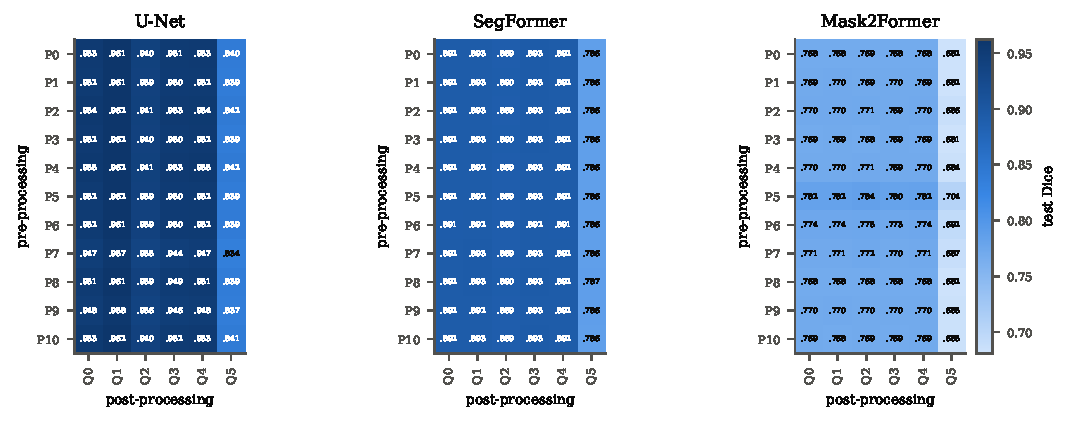
\includegraphics[width=0.82\textwidth]{heatmap_dice}
\caption{Test Dice of every combination of pre-processing (rows) and post-processing (columns) for each architecture. P0 and Q0 are the baselines.}
\label{fig:heat}
\end{figure*}

The configuration with the highest validation Dice among the 198 combinations, U-Net with RMS normalization and threshold optimization (E006), is reported in Table~\ref{tab:best_configuration}, and Table~\ref{tab:cross_dataset} gives the cross-dataset summary row of this dataset. Its relative gain of 0.95\% over U-Net alone depends on the initial snapshot, as examined in Section~\ref{subsec:sensitivity}.

\begin{table*}[t]
\centering
\caption{Best validation-selected configuration and held-out test performance. Selection criterion fixed before testing: highest mean validation Dice among all 198 combinations.}
\label{tab:best_configuration}
\small
\begin{tabularx}{\textwidth}{L{4.3cm} L{1.6cm} L{2.4cm} L{2.8cm} c c c}
\toprule
\textbf{Dataset} & \textbf{Architecture} & \textbf{Pre-processing} & \textbf{Post-processing} & \textbf{IoU} & \textbf{Dice} & \textbf{95\% CI (Dice)} \\
\midrule
\texttt{gray\_scott\_reaction\_}\newline\texttt{diffusion} & U-Net & P2 RMS & Q1 Threshold optim. & 0.950 & 0.962 & [0.960; 0.964] \\
\bottomrule
\end{tabularx}
\vspace{6pt}
\caption{Cross-dataset summary of the selected segmentation approach. Relative gain: test Dice of the selected configuration relative to the same architecture without pre- and post-processing.}
\label{tab:cross_dataset}
\small
\begin{tabularx}{\textwidth}{L{4.3cm} L{1.7cm} L{1.4cm} c c Y}
\toprule
\textbf{Dataset} & \textbf{Selected architecture} & \textbf{Selected P / Q} & \textbf{Test Dice} & \textbf{Relative gain (\%)} & \textbf{Generalization notes} \\
\midrule
\texttt{gray\_scott\_reaction\_}\newline\texttt{diffusion} & U-Net & P2 / Q1 & 0.962 & +0.95 & Gain over U-Net alone (0.953) comes from the random initial snapshot; for $n\geq50$, Dice 0.992 vs.\ 0.995 ($-$0.2\%). \\
\bottomrule
\end{tabularx}
\end{table*}


\subsection{Statistical reporting}\label{subsec:statistics}

All values are means over the 120 test trajectories, the statistical unit, with stratified bootstrap intervals (Section~\ref{subsec:cost}); adjacent frames of a trajectory are not treated as independent observations. With one seed per configuration, the intervals capture variability across test trajectories but not across training runs. The test split was not used to select thresholds, post-processing parameters or hyperparameters.

Table~\ref{tab:classwise_temporal} shows an aspect that the structure Dice does not reveal. For U-Net, threshold optimization raised the structure Dice but lowered the background IoU from 0.986 to 0.952 and the mIoU from 0.967 to 0.950; for SegFormer, the background IoU fell from 0.928 to 0.872, and the structure IoU fell by 1.18 points (Table~\ref{tab:prepost_effect}), while its Dice did not change. The trade-off comes from the threshold selected on validation, 0.2 for U-Net and SegFormer, which enlarges the region classified as structure.

\begin{table*}[t]
\centering
\caption{Class-wise and temporal metrics on the test set for the configurations of Table~\ref{tab:full_results}. IoU$_{bg}$, Dice$_{bg}$: background class; mIoU: mean IoU of the two classes; AVE: area-variation error (\% of the domain per sampled step); CDE: structure-centroid displacement error (pixels, periodic distance); TC: temporal consistency of the masks; TCE $=|\mathrm{TC}_{pred}-\mathrm{TC}_{GT}|$; memory: peak GPU memory at inference (batch 1). Mean $\pm$ half-width of the 95\% CI.}
\label{tab:classwise_temporal}
\scriptsize
\setlength{\tabcolsep}{3pt}
\begin{tabularx}{\textwidth}{L{0.7cm} L{1.6cm} Y c c c c c c c c}
\toprule
\textbf{ID} & \textbf{Architecture} & \textbf{Condition} & \textbf{IoU$_{bg}$} & \textbf{Dice$_{bg}$} & \textbf{mIoU} & \textbf{AVE (\%)} & \textbf{CDE (px)} & \textbf{TC} & \textbf{TCE} & \textbf{Mem. (MiB)} \\
\midrule
E151 & U-Net & Architecture only (P0+Q0) & 0.986{\scriptsize$\pm$0.001} & 0.992{\scriptsize$\pm$0.001} & 0.967{\scriptsize$\pm$0.001} & 0.76{\scriptsize$\pm$0.05} & 2.68{\scriptsize$\pm$0.34} & 0.686 & 0.010{\scriptsize$\pm$0.002} & 170 \\
E160 & U-Net & Pre + arch. (P4+Q0) & 0.986{\scriptsize$\pm$0.001} & 0.992{\scriptsize$\pm$0.001} & 0.967{\scriptsize$\pm$0.001} & 0.59{\scriptsize$\pm$0.07} & 2.16{\scriptsize$\pm$0.34} & 0.683 & 0.007{\scriptsize$\pm$0.001} & 170 \\
E152 & U-Net & Arch. + post (P0+Q1) & 0.952{\scriptsize$\pm$0.002} & 0.957{\scriptsize$\pm$0.002} & 0.950{\scriptsize$\pm$0.002} & 3.55{\scriptsize$\pm$0.14} & 1.57{\scriptsize$\pm$0.22} & 0.691 & 0.009{\scriptsize$\pm$0.001} & 170 \\
E006 & U-Net & Pre + arch. + post (P2+Q1) & 0.952{\scriptsize$\pm$0.002} & 0.957{\scriptsize$\pm$0.002} & 0.951{\scriptsize$\pm$0.002} & 3.58{\scriptsize$\pm$0.15} & 1.42{\scriptsize$\pm$0.21} & 0.691 & 0.008{\scriptsize$\pm$0.001} & 170 \\
\addlinespace
E167 & SegFormer & Architecture only (P0+Q0) & 0.928{\scriptsize$\pm$0.002} & 0.961{\scriptsize$\pm$0.001} & 0.883{\scriptsize$\pm$0.003} & 0.89{\scriptsize$\pm$0.05} & 7.16{\scriptsize$\pm$0.69} & 0.685 & 0.013{\scriptsize$\pm$0.002} & 227 \\
E180 & SegFormer & Pre + arch. (P8+Q0) & 0.929{\scriptsize$\pm$0.002} & 0.962{\scriptsize$\pm$0.001} & 0.883{\scriptsize$\pm$0.003} & 0.89{\scriptsize$\pm$0.05} & 7.18{\scriptsize$\pm$0.67} & 0.685 & 0.013{\scriptsize$\pm$0.002} & 227 \\
E168 & SegFormer & Arch. + post (P0+Q1) & 0.872{\scriptsize$\pm$0.002} & 0.912{\scriptsize$\pm$0.002} & 0.849{\scriptsize$\pm$0.003} & 3.87{\scriptsize$\pm$0.15} & 7.85{\scriptsize$\pm$0.62} & 0.698 & 0.014{\scriptsize$\pm$0.001} & 227 \\
E086 & SegFormer & Pre + arch. + post (P8+Q1) & 0.873{\scriptsize$\pm$0.002} & 0.912{\scriptsize$\pm$0.002} & 0.850{\scriptsize$\pm$0.003} & 3.87{\scriptsize$\pm$0.15} & 7.91{\scriptsize$\pm$0.60} & 0.697 & 0.014{\scriptsize$\pm$0.001} & 227 \\
\addlinespace
E183 & Mask2Former & Architecture only (P0+Q0) & 0.836{\scriptsize$\pm$0.007} & 0.908{\scriptsize$\pm$0.004} & 0.742{\scriptsize$\pm$0.008} & 1.20{\scriptsize$\pm$0.05} & 9.47{\scriptsize$\pm$0.64} & 0.686 & 0.014{\scriptsize$\pm$0.002} & 287 \\
E193 & Mask2Former & Pre + arch. (P5+Q0) & 0.796{\scriptsize$\pm$0.006} & 0.866{\scriptsize$\pm$0.003} & 0.727{\scriptsize$\pm$0.008} & 4.08{\scriptsize$\pm$0.14} & 7.13{\scriptsize$\pm$0.65} & 0.697 & 0.012{\scriptsize$\pm$0.001} & 287 \\
E185 & Mask2Former & Arch. + post (P0+Q2) & 0.839{\scriptsize$\pm$0.007} & 0.910{\scriptsize$\pm$0.004} & 0.744{\scriptsize$\pm$0.008} & 1.20{\scriptsize$\pm$0.05} & 9.95{\scriptsize$\pm$0.76} & 0.684 & 0.015{\scriptsize$\pm$0.002} & 287 \\
E122 & Mask2Former & Pre + arch. + post (P5+Q2) & 0.800{\scriptsize$\pm$0.006} & 0.869{\scriptsize$\pm$0.003} & 0.730{\scriptsize$\pm$0.008} & 4.10{\scriptsize$\pm$0.14} & 7.45{\scriptsize$\pm$0.81} & 0.695 & 0.010{\scriptsize$\pm$0.001} & 287 \\
\addlinespace
REF & Otsu on $A$ & Reference (P0+Q0) & 0.916{\scriptsize$\pm$0.005} & 0.951{\scriptsize$\pm$0.003} & 0.871{\scriptsize$\pm$0.008} & 1.76{\scriptsize$\pm$0.13} & 3.17{\scriptsize$\pm$0.43} & 0.710 & 0.027{\scriptsize$\pm$0.003} & n/a \\
\bottomrule
\end{tabularx}
\end{table*}


\subsection{Visual tables and temporal evolution}\label{subsec:visual}

Figs.~\ref{fig:vt_spirals} and \ref{fig:vt_gliders} show, for one test trajectory of two regimes, the initial snapshot ($n=0$), two intermediate snapshots and the final snapshot ($n=1000$). Snapshot $n=50$ is the first sampled after the initial condition and records the organization of the pattern, and $n=500$ is the characteristic frame on which the ground truth was defined. For each architecture, the figures show the input $A$, the input after the selected pre-processing, the ground truth and the masks of the four conditions. At $n=0$, the architectures without post-processing miss most of the ground truth, mostly with false negatives, whereas the configurations with a lowered threshold and Mask2Former with percentile clipping segment almost the whole domain, mostly with false positives. From $n=50$ onward, U-Net follows the structures with few errors, whereas SegFormer and Mask2Former concentrate errors at the boundaries.

\begin{figure*}[t]
\centering
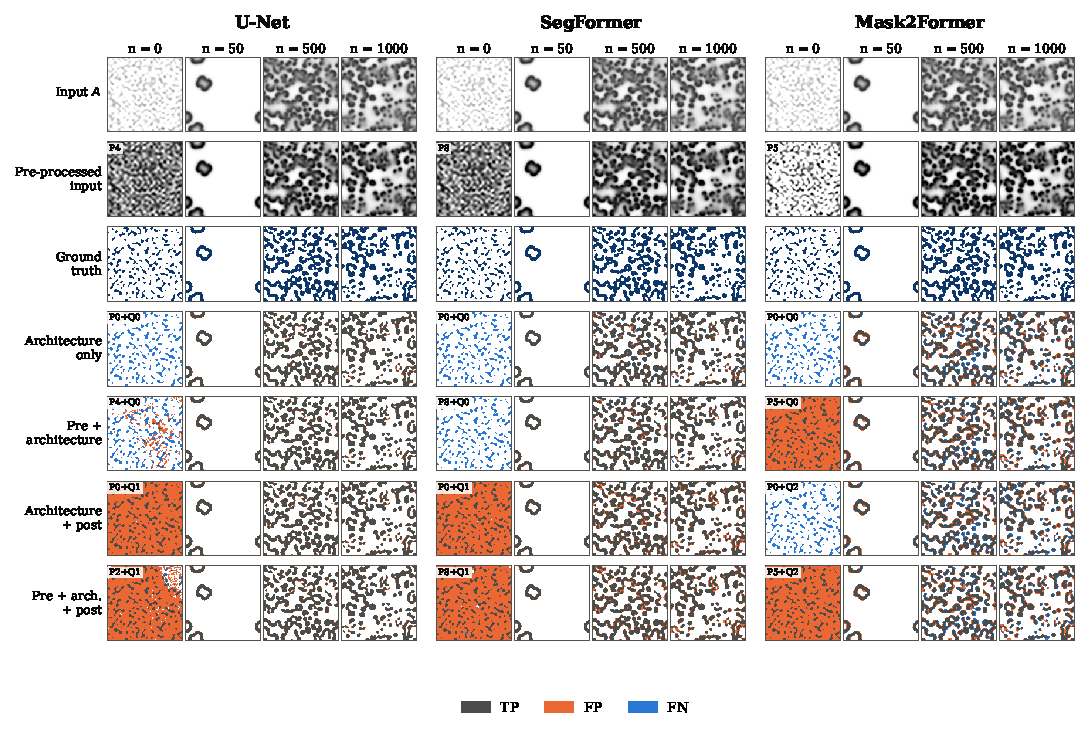
\includegraphics[width=0.84\textwidth]{visual_table_spirals}
\caption{Visual table, \textit{spirals} regime. For each architecture: input $A$, pre-processed input, ground truth and masks of the four conditions at $n=0$, $50$, $500$ and $1000$. Dark gray: true positive; orange: false positive; blue: false negative.}
\label{fig:vt_spirals}
\end{figure*}

\begin{figure*}[t]
\centering
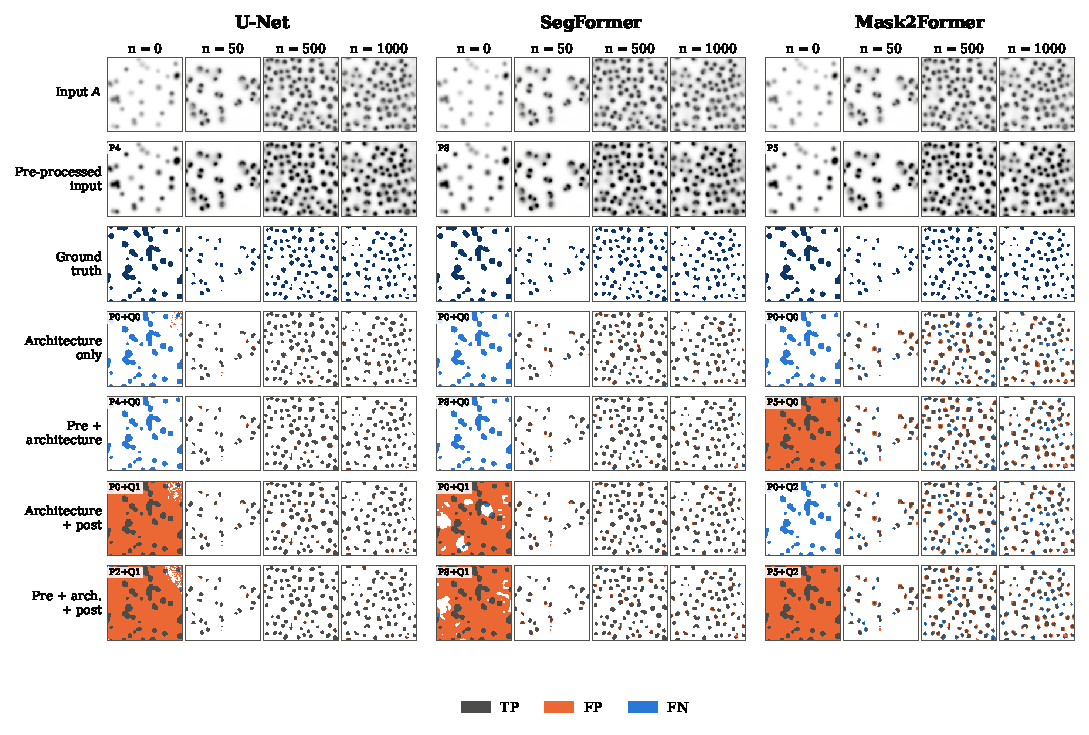
\includegraphics[width=0.84\textwidth]{visual_table_gliders}
\caption{Visual table, \textit{gliders} regime, with spots that move and split. Same layout as Fig.~\ref{fig:vt_spirals}.}
\label{fig:vt_gliders}
\end{figure*}

At $n=50$, U-Net alone already reached a Dice of 0.994, SegFormer 0.952 and Mask2Former 0.829, and from $n=100$ onward the means were 0.995, 0.930 and 0.800 (Fig.~\ref{fig:temporal}); the reference reached 0.869 at $n=50$ and 0.923 from $n=100$ onward. U-Net alone had the lowest area-variation error, 0.76\% of the domain per sampled step, and a TCE of 0.010 for a ground-truth consistency of 0.689 (Table~\ref{tab:classwise_temporal}). Its final configuration (P2+Q1) lowered the centroid error from 2.68 to 1.42 pixels but raised the area-variation error to 3.58\%, an effect of the area jump between the over-segmented initial snapshot and the following ones. SegFormer and Mask2Former kept centroid errors of 7.1 to 10.0 pixels. U-Net thus followed the evolution of the structures from the first sampled snapshot after the initial condition, whereas no configuration segmented the initial snapshot informatively (RQ4).

\begin{figure}[t]
\centering
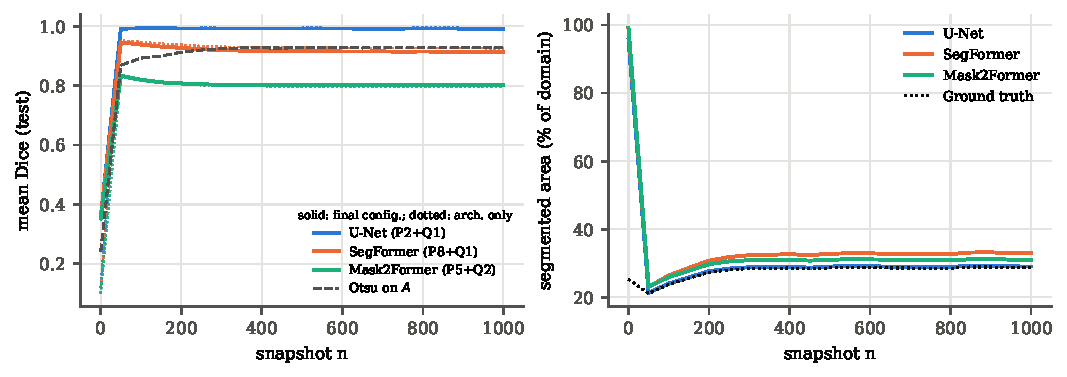
\includegraphics[width=\columnwidth]{temporal_dice_area}
\caption{Left: mean test Dice per snapshot for the final configuration of each architecture (solid), the architecture alone (dotted) and Otsu on $A$ (dashed). Right: mean segmented area (\% of the domain).}
\label{fig:temporal}
\end{figure}

\subsection{Sensitivity to the initial snapshot}\label{subsec:sensitivity}

Snapshot $n=0$ is one of the 21 sampled snapshots, and its initial condition is random. Table~\ref{tab:sensitivity} separates its Dice from that of the other snapshots. The architectures without post-processing obtained a Dice between 0.100 and 0.120 at $n=0$, with U-Net predicting about 11\% of the domain against 25.3\% in the ground truth. With the 0.2 threshold, U-Net segmented 95.2\% of the domain at that snapshot, and its Dice rose to 0.353. Over $n\geq50$, however, P2+Q1 reached 0.992, below the 0.995 of U-Net alone. Recomputed without the initial snapshot, the paired effect of threshold optimization changed sign: $-0.28$ point for U-Net and $-1.21$ for SegFormer, both distinguishable from zero (Table~\ref{tab:prepost_effect}). The effect of percentile clipping on Mask2Former fell from 1.37 to 0.18 points, since that configuration also predicted 99.2\% of the domain at $n=0$. The effects of opening and temporal filtering kept their sign and magnitude. Without the initial snapshot, SegFormer reached 0.931, above the 0.921 of the reference.

\begin{table}[t]
\centering
\caption{Sensitivity to the initial snapshot: mean test Dice over all 21 snapshots, at the random initial snapshot $n=0$ only and over the 20 snapshots $n\geq50$.}
\label{tab:sensitivity}
\scriptsize
\setlength{\tabcolsep}{3pt}
\begin{tabularx}{\columnwidth}{L{0.7cm} Y c c c}
\toprule
\textbf{ID} & \textbf{Configuration} & \textbf{All} & \textbf{$n=0$} & \textbf{$n\geq50$} \\
\midrule
E151 & U-Net (P0+Q0) & 0.953 & 0.120 & 0.995 \\
E160 & U-Net (P4+Q0) & 0.955 & 0.153 & 0.995 \\
E152 & U-Net (P0+Q1) & 0.961 & 0.353 & 0.992 \\
E006 & U-Net (P2+Q1) & 0.962 & 0.354 & 0.992 \\
\addlinespace
E167 & SegFormer (P0+Q0) & 0.892 & 0.100 & 0.931 \\
E180 & SegFormer (P8+Q0) & 0.892 & 0.100 & 0.932 \\
E168 & SegFormer (P0+Q1) & 0.893 & 0.357 & 0.919 \\
E086 & SegFormer (P8+Q1) & 0.893 & 0.357 & 0.920 \\
\addlinespace
E183 & Mask2Former (P0+Q0) & 0.768 & 0.102 & 0.801 \\
E193 & Mask2Former (P5+Q0) & 0.782 & 0.353 & 0.803 \\
E185 & Mask2Former (P0+Q2) & 0.769 & 0.101 & 0.802 \\
E122 & Mask2Former (P5+Q2) & 0.784 & 0.353 & 0.805 \\
\addlinespace
REF & Otsu on $A$ (P0+Q0) & 0.888 & 0.241 & 0.921 \\
\bottomrule
\end{tabularx}
\end{table}


\subsection{Pattern regimes and computational cost}\label{subsec:regimes}

U-Net alone kept a Dice between 0.943 and 0.979 in all regimes (Table~\ref{tab:regime}). SegFormer had its lowest values in \textit{spots} (0.833), \textit{maze} (0.865) and \textit{worms} (0.868), below the 0.906, 0.938 and 0.896 of the reference in these regimes, which are those with the shortest wavelengths (Table~\ref{tab:regimes}); Mask2Former also had its lowest value in \textit{spots} (0.667).

\begin{table}[t]
\centering
\caption{Test Dice per pattern regime (20 test trajectories each) for each architecture alone, for its validation-selected pre- + post-processing pair and for the learning-free reference.}
\label{tab:regime}
\scriptsize
\setlength{\tabcolsep}{2.5pt}
\begin{tabularx}{\columnwidth}{Y *{6}{c}}
\toprule
\textbf{Configuration} & \textbf{Glid.} & \textbf{Bubb.} & \textbf{Maze} & \textbf{Worms} & \textbf{Spir.} & \textbf{Spots} \\
\midrule
U-Net (P0+Q0) & 0.948 & 0.979 & 0.950 & 0.948 & 0.943 & 0.949 \\
U-Net (P2+Q1) & 0.963 & 0.981 & 0.959 & 0.956 & 0.955 & 0.958 \\
SegFormer (P0+Q0) & 0.927 & 0.952 & 0.865 & 0.868 & 0.905 & 0.833 \\
SegFormer (P8+Q1) & 0.941 & 0.952 & 0.859 & 0.866 & 0.912 & 0.829 \\
Mask2Former (P0+Q0) & 0.833 & 0.800 & 0.781 & 0.712 & 0.816 & 0.667 \\
Mask2Former (P5+Q2) & 0.850 & 0.803 & 0.795 & 0.726 & 0.835 & 0.692 \\
Otsu on $A$ (P0+Q0) & 0.852 & 0.917 & 0.938 & 0.896 & 0.821 & 0.906 \\
\bottomrule
\end{tabularx}
\end{table}

\begin{table}[t]
\centering
\caption{Model size and cost (20 epochs, batch 32, native $128\times128$ input, reference input P0). Best epoch: epoch of the checkpoint with the highest validation Dice, range over the 11 inputs P0 to P10. Latency and throughput measured with a dedicated GPU after all training runs.}
\label{tab:cost}
\scriptsize
\setlength{\tabcolsep}{3pt}
\begin{tabularx}{\columnwidth}{Y c c c c c}
\toprule
\textbf{Architecture} & \textbf{Params (M)} & \textbf{Train (min)} & \textbf{Best epoch} & \textbf{Latency (ms)} & \textbf{fps} \\
\midrule
U-Net & 24.4 & 21 & 11 to 20 & 5.58 & 4932 \\
SegFormer & 27.3 & 35 & 19 to 20 & 15.61 & 2073 \\
Mask2Former & 47.4 & 273 & 1 to 9 & 38.63 & 552 \\
\bottomrule
\end{tabularx}
\end{table}


U-Net had the lowest latency (5.58~ms) and the shortest training, whereas Mask2Former, with 47.4 million parameters, had a latency of 38.63~ms and the longest training under shared execution (Table~\ref{tab:cost}). The selected epoch also differed: for SegFormer it was epoch 19 or 20 for every input, which indicates that its validation Dice was still increasing at the end of the budget; for Mask2Former it was between epochs 1 and 9, since its validation Dice stayed between 0.771 and 0.776 over the 20 epochs for the reference input.

%% ============================================================================
\section{Discussion, applicability and limitations}\label{sec:sec6}

\subsection{Architectures and output resolution}\label{subsec:disc_arch}

The ranking of the architectures was determined by a design property, the output resolution, more than by the techniques applied before or after the network. U-Net predicts at the input resolution, with skip connections from the highest-resolution stage, whereas SegFormer and Mask2Former predict on $32\times32$ cells for a $128\times128$ input. With structures a few pixels in diameter (Table~\ref{tab:regimes}), one output cell of these architectures covers a considerable part of a structure, and the boundary depends on the interpolation of the logits. This interpretation is consistent with the drop of SegFormer in the regimes with the shortest wavelengths, where it fell below the thresholding of $A$. The design, however, does not isolate output resolution from other differences between the architectures, such as backbone and pre-training.

Mask2Former should be read with caution. Its validation Dice plateaued in the first epochs while the training loss kept decreasing, which is consistent with two hypotheses that the design does not separate: the low-resolution output and the training without deep supervision, part of the original recipe~\cite{cheng2022mask2former}. Its mask-classification formulation was also conceived for objects of natural scenes, whereas here one class is spread over tens of disconnected components. Its results therefore characterize the configuration actually trained, not the potential of the architecture. For SegFormer, the best epoch at the end of the budget indicates that the 20-epoch limit may have constrained it.

\subsection{Why pre- and post-processing helped or hurt}\label{subsec:disc_why}

The small effect of pre-processing is consistent with the properties of the data. Simulated fields contain no acquisition noise, so denoising filters have little to remove, while smoothing filters remove signal: Gaussian smoothing attenuates the harmonics that define sharp boundaries, and the median filter rounds corners and removes one-pixel necks. This loss of detail is consistent with the losses observed for U-Net, the only architecture able to exploit that detail. Normalizations are, to first order, affine transformations whose effect tends to be absorbed by the normalization layers of the networks, which is consistent with effects close to zero.

Post-processing effects followed the scale of the operations relative to the structures and to the temporal sampling. Opening with a radius-1 disk removes structures less than three pixels wide, such as nascent spots and the thin walls of \textit{bubbles}, which U-Net already preserved. That connected-component filtering changed nothing is consistent with networks applied to smooth fields hardly producing isolated specks, so the point-noise hypothesis behind the method did not hold here. Temporal filtering combines snapshots 500 time units apart; where the pattern moves, structures change position within that interval, and the median produces lagged masks that erase real physical changes, consistent with losses of about 30 points in \textit{gliders} and \textit{spirals} and with the caveat of the protocol about this method.

\subsection{Selection criterion and the initial snapshot}\label{subsec:disc_n0}

The sensitivity to the initial snapshot is the result with the largest methodological consequence. At $n=0$, the initial condition is random, and $A$ does not yet reflect the structure of $B$, so no configuration segmented that snapshot informatively. Still, one snapshot out of 21 was enough to decide the selection on validation: a low threshold makes the network segment almost the whole domain at $n=0$, which raises the Dice of that frame without any physical information, and the same effect explains most of the gain of percentile clipping on Mask2Former. Over the snapshots with a pattern, threshold optimization lowered the Dice of U-Net and SegFormer and lowered the background IoU, which shows that the mean structure Dice, used as the single selection criterion, favored over-segmenting an uninformative frame. Choosing a configuration to follow the evolution of the structures should therefore consider class-wise and temporal metrics and exclude or down-weight the initial snapshot when the initial condition is random. Other datasets of the class with random or structureless initial conditions may be subject to the same effect when their results are merged.

\subsection{Applicability and real-time feasibility}\label{subsec:disc_realtime}

With 5.58~ms per $128\times128$ frame, U-Net segments about 180 frames per second at batch 1 and about 4,900 in batches, so a full trajectory of 1,001 snapshots takes under a second. This cost is compatible with monitoring a simulation or a neural surrogate while it runs, for example, to track the active-reaction area of a reactor model or the extent of a simulated release. The learning-free reference is about 18 times faster (0.30~ms) but loses 6.5 points of Dice over all snapshots and 7.4 over those with a pattern; post-processing added at most 0.51~ms per frame. These figures refer to one GPU and batch 1 after warm-up.

\subsection{Limitations}\label{subsec:limitations}

Regarding internal validity, each configuration was trained with one seed, Mask2Former without deep supervision, and the architectures differ simultaneously in output resolution, backbone and pre-training, so no comparison between them identifies the cause of the differences; the training runs also shared the GPU, which affects training times but not the latencies. Regarding construct validity, the ground truth was defined by thresholding $B$, not by expert annotation, and depends on the reference snapshot and on the Otsu criterion, so the experiment measures the recovery of a physically defined segmentation; the anti-correlation between $A$ and $B$ makes the task simpler than natural-image segmentation, which is why the learning-free reference was included; and the stride of 50 snapshots limits the temporal resolution of the evolution metrics. Regarding external validity, the results refer to one physical system, one GPU and frame-wise networks.

%% ============================================================================
\section{Conclusions}\label{sec:conclusions}

This study evaluated pre-processing, architecture and post-processing for the temporal segmentation of the active-reaction regions of the Gray-Scott system of The Well, under the common protocol of the class. U-Net reached a Dice of 0.953 without pre- or post-processing, above the Otsu reference on $A$ (0.888), whereas SegFormer was not distinguishable from that reference (0.892) and Mask2Former stayed below it (0.768). Pre-processing changed Dice by at most 1.37 percentage points, the largest effect being driven by the initial snapshot. Threshold optimization raised the mean Dice of U-Net by 0.84 points but lowered it once the initial snapshot was excluded, and temporal consistency filtering lowered the Dice of all architectures by 8.6 to 11.3 points, with losses of about 30 points in the regimes whose structures move. U-Net followed the evolution of the structures from the first sampled snapshot, with a mean Dice of 0.995 from $n=100$ onward, but no configuration segmented the random initial snapshot. In this dataset, the output resolution of the architecture weighed more than the techniques applied before and after it, and selecting configurations by mean Dice was sensitive to a single frame without physical information.

Further work requires more seeds, Mask2Former with deep supervision, Transformer architectures with varied output resolution, a selection criterion that excludes or down-weights the initial snapshot, temporal architectures, and the merging of these results with those of the other datasets of the class.

%% ============================================================================
%% SECOES FINAIS OBRIGATORIAS (BACKMATTER)
%% ============================================================================
\section*{CRediT authorship contribution statement}
%% Papeis CRediT de cada autor: confirmar com os autores antes da entrega.
\textbf{Andre Luis Aguiar do Nascimento:} [roles to be defined].
\textbf{Joao Guilherme Miranda Lago:} [roles to be defined].
\textbf{Wesley dos Santos Gatinho:} Conceptualization, Methodology, Software, Investigation, Formal analysis, Data curation, Visualization, Writing (original draft), Writing (review \& editing).

\section*{Declaration of competing interest}
The authors declare no known competing financial interests or personal relationships that could have appeared to influence the work reported in this paper.

\section*{Data availability}
The data are publicly available from The Well (\url{https://polymathic-ai.org/the_well/}). The trajectory identifiers, the per-combination results (\texttt{results\_sequential.csv}, \texttt{results\_protocolo.csv}) and the code that downloads the subset, builds the ground truth, trains the models and generates every table and figure are available from the authors.

%% ============================================================================
%% REFERENCIAS (Estilo numerico Elsevier: elsarticle-num)
%% ============================================================================
\setlength{\bibsep}{1pt plus 0.5pt}
\bibliographystyle{elsarticle-num}
\bibliography{references}

\end{document}
